% !tex root = 01.tcp.file.transfer.tex
\documentclass{article}
\usepackage{hyperref}
\usepackage{bookmark}
\usepackage[utf8]{inputenc}
\usepackage{geometry}
 \geometry{
 a4paper,
 total={170mm,257mm},
 left=20mm,
 top=20mm,
 }
\usepackage{graphicx}
\usepackage{float}
\usepackage{caption}
\captionsetup[figure]{
    position=below,
}
\usepackage{titling}

\title{A simple TCP system capable of transfering files
}

\usepackage{listings}
\usepackage{color}

\definecolor{dkgreen}{rgb}{0,0.6,0}
\definecolor{gray}{rgb}{0.5,0.5,0.5}
\definecolor{mauve}{rgb}{0.58,0,0.82}
\definecolor{blue}{rgb}{1,0,0}
\hypersetup{
    colorlinks=true,
    linkcolor=blue,
    filecolor=magenta,      
    urlcolor=cyan,
    pdfpagemode=FullScreen,
    }

\lstset{frame=tb,
  language=Python,
  aboveskip=3mm,
  belowskip=3mm,
  showstringspaces=false,
  columns=flexible,
  basicstyle={\small\ttfamily},
  numbers=none,
  numberstyle=\tiny\color{gray},
  keywordstyle=\color{blue},
  commentstyle=\color{dkgreen},
  stringstyle=\color{mauve},
  breaklines=true,
  breakatwhitespace=true,
  tabsize=3
}

\author{Nguyen Trong Minh}
\date{November 2024}
 
 \usepackage{fancyhdr}
\pagestyle{fancyplain}
\fancyhf{} % clear all header and footer fields
\fancyfoot[R]{
\includegraphics[width=2cm]{usth.png}}
\fancyfoot[L]{\thedate}
\fancyhead[L]{Practical 1}
\fancyhead[R]{\theauthor}

\usepackage{fancyvrb}
\makeatletter
\def\@maketitle{%
  \newpage
  \null
  \vskip 1em%
  \begin{center}%
  \let \footnote \thanks
    {\LARGE \@title \par}%
    \vskip 1em%
    %{\large \@date}%
  \end{center}%
  \par
  \vskip 1em}
\makeatother

\usepackage{lipsum}  
\usepackage{cmbright}

\begin{document}

\maketitle

\noindent\begin{tabular}{@{}ll}
     Developer &  \theauthor \\
     Report writer & \theauthor
\end{tabular}

\section*{System design}
As mentioned in the assignment, we created a system consists of 2 members, a server and a client. 
We also created a file to import constants used in our system.
\begin{lstlisting}[frame=single]
  HOST = '127.0.0.1'
  PORT = 8080
  TOTALCLIENTS = 1
  BUFFERSIZE = 1024
  
  class Signal(Enum):
      CLOSE_SERVER = b'CLS'
      SEND_A_FILE = b'SAF'
      REQUEST_A_FILE = b'RAF'
      SEND_A_REPO = b'SAR'
      REQUEST_A_REPO = b'RAR'
      DONE = b'DON'
      ERROR = b'ERR'
      PING = b'PIN'
      PONG = b'PON'
  
  SIGNALSIZE = getsizeof(Signal.CLOSE_SERVER.value)
\end{lstlisting}
The code above also revealed functions exists in our system that we will go into further detail later.
For the system design, you can see that we created Signal class to store signal used in communication between server and client.
We introduced 5 signals for noticing server about what is going to happen from client side $\texttt{CLOSE\_SERVER, SEND\_A\_FILE, SEND\_A\_REPO, REQUEST\_ A\_FILE, REQUEST\_A\_REPO}$ 
and 4 signals to communicate between server and client $ \texttt{DONE, ERROR, PING, PONG}$. We also fixed size of each bytes buffer to be sent for files' content at 1024 bytes, and for signal is the size of 36 bytes. \\
\\
Our server first bind itself to a port, in our case 127.0.0.1:8080, it then start listening to any connection from client, which is 1 only. 
\begin{lstlisting}[frame=single]
  sock = socket.socket(socket.AF_INET, socket.SOCK_STREAM) 
  sock.bind((HOST, PORT)) 
  sock.listen(TOTALCLIENTS) 

  # Establishing Connections 
  client_socket, clar = sock.accept()
\end{lstlisting}
At this point we used a loop to check if the client has sent any signal to the server to send or request any file. We have 4 functions to send and receive any file as requseted from client.
If the signal sent from client match specific signal addressed for each function, the server executes it. \pagebreak
\begin{lstlisting}[frame=single]
  while True:
    sig = receive_signal(client_socket)
    if sig == Signal.CLOSE_SERVER.value:
        print('closing')
        break
    if sig == Signal.SEND_A_FILE.value:
        receive_file(client_socket, file_name=r'file-transfered/server-receive/recv0.txt')
    if sig == Signal.REQUEST_A_FILE.value:
        file_name = client_socket.recv(BUFFERSIZE)
        send_file(client_socket, file_name.decode())
    if sig == Signal.SEND_A_REPO.value:
        receive_repo(client_socket, r'file-transfered/server-receive/')
    if sig == Signal.REQUEST_A_REPO.value:
        repo_name = client_socket.recv(BUFFERSIZE)
        send_repo(client_socket, repo_name.decode())
    if not sig:
        break
    print(sig.decode())
\end{lstlisting} 
With the client, it is simply a sequential code to execute specific task that we defined inside \hyperref[functions]{Function desgin}.
After all, take a look at our server workflow graph:
\begin{figure}[H]
  \centering
  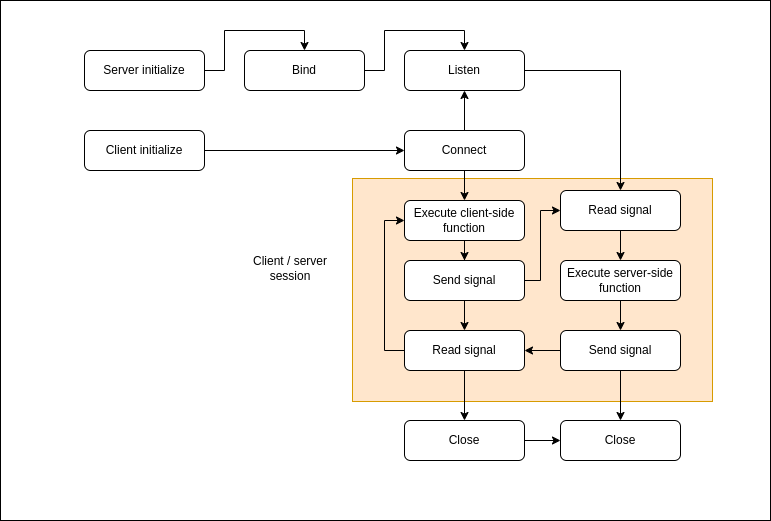
\includegraphics[scale=0.6]{TCP_server.png}
  \caption{Overall workflow of TCP system}
\end{figure}

\section*{Functions design}\label{functions}

In this section, we will go through 4 functions designed to send 1 or more files between server and client in our system. 

\subsection*{Send a file from client to server}
The first funtion is to send a single file from client to server, we start by take a look at client-side code: \pagebreak
\begin{lstlisting}[frame=single]
  def send_file(client_socket : socket.socket, file_name: str):
    """Send a file to server"""
    if not exists(file_name):
        raise FileNotFoundError(f'{file_name} does not exist')
    
    send_signal(client_socket, Signal.SEND_A_FILE )
    sleep(0.1)
    
    client_socket.send(file_name.split("/")[-1].encode())
    sleep(0.1)

    with open(file_name, 'rb') as f:
        while chunk := f.read(BUFFERSIZE):
            client_socket.send(chunk)

    sleep(0.1)
    send_signal(client_socket, Signal.DONE)
\end{lstlisting}
We first make sure the file we want to send is visible by the client object, then we send a $ \texttt{SEND\_A\_FILE} $ signal to let the sever know 
that we are going to send a file and it have to ready to receive for it. Next step, we send file name to the server in case the server does not have 
a specific name to save this file, it will use the name provided by client. After that, we read file content by chunk of size 1024 bytes and send each to
server until there are nothing left. At the end, send a $ \texttt{DONE} $ signal to confirm that we have sent everything. On the other side, the server 
also run a sequential actions to read everything sent by client. 
\begin{lstlisting}[frame=single]
  def receive_file(
    client_socket: socket.socket, 
    file_name: str | None = None, 
    repo_to_save: str | None = None
    ) -> None:
  """Receives a file from the client."""

  # Get file name from client side
  clif_name = client_socket.recv(BUFFERSIZE)
  clif_name = clif_name.decode()

  if file_name is None: file_name = clif_name
  if repo_to_save is not None: file_name = os.path.join(repo_to_save, file_name)

  with open(file_name, 'wb') as file:
      print(f"Receiving file: {clif_name}")
      while True:
          data = client_socket.recv(BUFFERSIZE)

          if not data or data == Signal.DONE.value:  # End signal
              break
          file.write(data)

  print(f"File received: {file_name}")
\end{lstlisting}
Quickly go through the code, we read file name sent by client, use it to save file in case save path is not specified, and then write every chunk of information
into a new file, in this case is a text file.
\subsection*{Request a file from server by client}
This function is used to request for any file stored on the server. The client first sends a signal to notice the server that it needs to download a file, then
sends the requested file name to server. And then waits for the server to respond with file content. We also have a litle signal "ping-pong" between server and client
to make sure the connection is secured during the process.\pagebreak
\begin{lstlisting}[frame=single]
  def request_file(client_socket : socket.socket, file_name: str, save_file=None):
    """Request a file from server"""
    if save_file is None: save_file = file_name

    send_signal(client_socket, Signal.REQUEST_A_FILE )
    sleep(0.1)
    client_socket.send(file_name.encode())
    sleep(0.1)

    response = recv_signal(client_socket)
    if response == Signal.ERROR.value:
        print("Error: File not found")
        return None
     
    with open(save_file, 'wb') as file:
        print(f"Downloading file: {file_name}")
        while True:
            data = client_socket.recv(BUFFERSIZE)
            send_signal(client_socket, Signal.PONG)

            if not data or data == Signal.DONE.value:  # End signal
                break

            file.write(data)
\end{lstlisting}
On the server-side, it receives name of the requested file outside the function, and then passes it into the function below:
\begin{lstlisting}[frame=single]
  def send_file(
        client_socket: socket.socket, 
        file_name: str
        ) -> None:
    """Sends a file to the client."""
    if os.path.exists(file_name):
        print(f"Sending file: {file_name}")

        with open(file_name, 'rb') as file:
            while chunk := file.read(BUFFERSIZE):
                send_signal(client_socket, Signal.PING)
                sleep(0.1)
                client_socket.send(chunk)

        sleep(0.1)
        send_signal(client_socket, Signal.DONE)  # End signal

        print("File sent successfully.")
    else:
        client_socket.send(b'ERROR: File not found')
        print("File not found.")
\end{lstlisting}
Because the client already know about what is going on, the server checks file existance and sends it back right away. If the requested file is not exist,
the server will send back an $ \texttt{ERROR}$ signal. As mentioned above, we have a "ping-pong" interaction between server and client between each chunk 
being sent. After transfering file content, our server sends a $\texttt{DONE}$ signal as confirmation. 

\begin{figure}[H]
  \centering
  \begin{minipage}{0.45\textwidth}
      \centering
      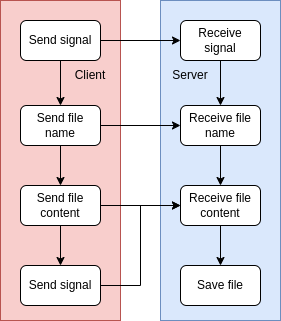
\includegraphics[width=0.93\textwidth]{SEND_A_FILE.drawio.png} % first figure itself
      \caption{Send a file workflow}
  \end{minipage}\hfill
  \begin{minipage}{0.45\textwidth}
      \centering
      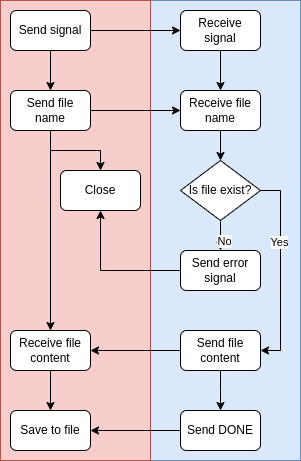
\includegraphics[width=0.7\textwidth]{REQUEST_A_FILE.drawio.png} % second figure itself
      \caption{Request a file workflow}
  \end{minipage}
\end{figure}

\subsection*{Send and request a repository}
These 2 functons are just stack of multiple send a file function together to send multiple files inside a repository so I'll quickly provide 2 workflow charts
for this part.

\begin{figure}[H]
  \centering
  \begin{minipage}{0.45\textwidth}
      \centering
      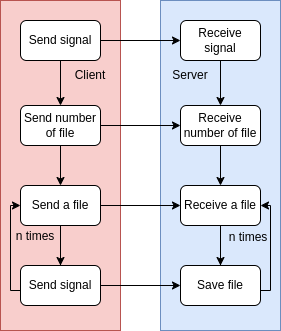
\includegraphics[width=0.9\textwidth]{SEND_A_REPO.drawio.png} % first figure itself
      \caption{Send a repository workflow}
  \end{minipage}\hfill
  \begin{minipage}{0.45\textwidth}
      \centering
      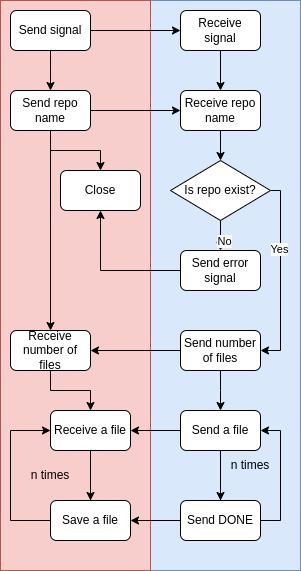
\includegraphics[width=0.9\textwidth]{REQUEST_A_REPO.drawio.png} % second figure itself
      \caption{Request a repository workflow}
  \end{minipage}
\end{figure}
\pagebreak
\section*{Other works}
We created a simple code to generate random content for text files to test our system in transfering files.

\begin{lstlisting}[frame=single]
  from os.path import join
  import random
  import lorem

  random.seed(4090)
  root = r'file-transfered'
  dirs = ['client-send', 'server-send']

  for dir in dirs:
    dir = join(root,dir)
    for i in range(1,10):
      with open(join(dir, f'dummy{i}.txt'), 'w') as f:
        random_text = lorem.paragraph()
        f.write(random_text)
\end{lstlisting}
\end{document}
